\documentclass[a4paper]{article}
\usepackage{times}
\usepackage[utf8]{inputenc}
\usepackage{selinput}
\usepackage{upquote}
\usepackage[margin=2cm, rmargin=4cm, tmargin=3cm]{geometry}
\usepackage{tcolorbox}
\usepackage{xspace}
\usepackage[french]{babel}
\usepackage{url}
\usepackage{hyperref}
\usepackage{fontawesome5}
\usepackage{marginnote}
\usepackage{ulem}
\usepackage{tcolorbox}
\usepackage{graphicx}
%\usepackage[top=Bcm, bottom=Hcm, outer=Ccm, inner=Acm, heightrounded, marginparwidth=Ecm, marginparsep=Dcm]{geometry}


\newtcolorbox{Example}[1]{colback=white,left=20pt,colframe=slideblue,fonttitle=\bfseries,title=#1}
\newtcolorbox{Solutions}[1]{colback=white,left=20pt,colframe=green,fonttitle=\bfseries,title=#1}
\newtcolorbox{Conseils}[1]{colback=white,left=20pt,colframe=slideblue,fonttitle=\bfseries,title=#1}
\newtcolorbox{Warning}[1]{colback=white,left=20pt,colframe=warning,fonttitle=\bfseries,title=#1}

\setlength\parindent{0pt}

  %Exercice environment
  \newcounter{exercice}
  \newenvironment{Exercice}[1][]
  {
  \par
  \stepcounter{exercice}\textbf{Question \arabic{exercice}:} (\faClock \enskip \textit{#1})
  }
  {\bigskip}
  

% Title
\newcommand{\titre}{\begin{center}
  \section*{Algorithmes et Pensée Computationnelle}
\end{center}}
\newcommand{\cours}[1]
{\begin{center} 
  \textit{#1}\\
\end{center}
  }


\newcommand{\exemple}[1]{\newline~\textbf{Exemple :} #1}
%\newcommand{\attention}[1]{\newline\faExclamationTriangle~\textbf{Attention :} #1}

% Documentation url (escape \# in the TP document)
\newcommand{\documentation}[1]{\faBookOpen~Documentation : \href{#1}{#1}}

% Clef API
\newcommand{\apikey}[1]{\faKey~Clé API : \lstinline{#1}}
\newcommand{\apiendpoint}[1]{\faGlobe~Url de base de l'API \href{#1}{#1}}

%Listing Python style
\usepackage{color}
\definecolor{slideblue}{RGB}{33,131,189}
\definecolor{green}{RGB}{0,190,100}
\definecolor{blue}{RGB}{121,142,213}
\definecolor{grey}{RGB}{120,120,120}
\definecolor{warning}{RGB}{235,186,1}

\usepackage{listings}
\lstdefinelanguage{texte}{
    keywordstyle=\color{black},
    numbers=none,
    frame=none,
    literate=
           {é}{{\'e}}1
           {è}{{\`e}}1
           {ê}{{\^e}}1
           {à}{{\`a}}1
           {â}{{\^a}}1
           {ù}{{\`u}}1
           {ü}{{\"u}}1
           {î}{{\^i}}1
           {ï}{{\"i}}1
           {ë}{{\"e}}1
           {Ç}{{\,C}}1
           {ç}{{\,c}}1,
    columns=fullflexible,keepspaces,
	breaklines=true,
	breakatwhitespace=true,
}
\lstset{
    language=Python,
	basicstyle=\bfseries\footnotesize,
	breaklines=true,
	breakatwhitespace=true,
	commentstyle=\color{grey},
	stringstyle=\color{slideblue},
  keywordstyle=\color{slideblue},
	morekeywords={with, as, True, False, Float, join, None, main, argparse, self, sort, __eq__, __add__, __ne__, __radd__, __del__, __ge__, __gt__, split, os, endswith, is_file, scandir, @classmethod},
	deletekeywords={id},
	showspaces=false,
	showstringspaces=false,
	columns=fullflexible,keepspaces,
	literate=
           {é}{{\'e}}1
           {è}{{\`e}}1
           {ê}{{\^e}}1
           {à}{{\`a}}1
           {â}{{\^a}}1
           {ù}{{\`u}}1
           {ü}{{\"u}}1
           {î}{{\^i}}1
           {ï}{{\"i}}1
           {ë}{{\"e}}1
           {Ç}{{\,C}}1
           {ç}{{\,c}}1,
    numbers=left,
}

\newtcbox{\mybox}{nobeforeafter,colframe=white,colback=slideblue,boxrule=0.5pt,arc=1.5pt, boxsep=0pt,left=2pt,right=2pt,top=2pt,bottom=2pt,tcbox raise base}
\newcommand{\projet}{\mybox{\textcolor{white}{\small projet}}\xspace}
\newcommand{\optionnel}{\mybox{\textcolor{white}{\small Optionnel}}\xspace}
\newcommand{\advanced}{\mybox{\textcolor{white}{\small Pour aller plus loin}}\xspace}
\newcommand{\auto}{\mybox{\textcolor{white}{\small Auto-évaluation}}\xspace}


\usepackage{environ}
\newif\ifShowSolution
\NewEnviron{solution}{
  \ifShowSolution
	\begin{Solutions}{\faTerminal \enskip Solution}
		\BODY
	\end{Solutions}
  \fi}


  \usepackage{environ}
  \newif\ifShowConseil
  \NewEnviron{conseil}{
    \ifShowConseil
    \begin{Conseils}{\faLightbulb \quad Conseil}
      \BODY
    \end{Conseils}

    \fi}

    \usepackage{environ}
  \newif\ifShowWarning
  \NewEnviron{attention}{
    \ifShowWarning
    \begin{Warning}{\faExclamationTriangle \quad Attention}
      \BODY
    \end{Warning}

    \fi}
  

%\newcommand{\Conseil}[1]{\ifShowIndice\ \newline\faLightbulb[regular]~#1\fi}


\usepackage{array}
\usepackage{amsmath}
\usepackage{tabto}
\newcolumntype{C}[1]{>{\centering\let\newline\\\arraybackslash\hspace{0pt}}m{#1}}

\begin{document}

% Change the following values to true to show the solutions or/and the hints
\ShowSolutiontrue
\ShowConseiltrue
\titre
\cours{Spatial Algorithms}

Le but de cette séance est de comprendre les algorithmes probabilistes. Ceux-ci permettent de résoudre des problèmes complexes de en relativement peu de temps. La contrepartie est que le résultat obtenu est généralement une solution approximée du problème initial. Ils demeurent néanmoins très utile pour beaucoup d'application.

\section{Monte-Carlo}
\begin{Exercice}[10 minutes]\textbf{Un jeu de hasard : Python}\\
Supposez que vous lanciez une pièce de monnaie l fois et que vous voulez calculez la probabilité d'avoir un certains nombre de pile. Vous devez programmer un algorithme probabiliste, permettant de calculer cette probabilité. Pour ce faire, vous devez compléter la fonction \textit{proba(n,l,iter)} contenue dans le fichier Piece.py. La fonction \textit{Piece(l)} permet de créer une liste contenant des 0 et des 1 aléatoirement avec une probabilité $\frac{1}{2}$. Considérez un chiffre 1 comme une réussite (pile) et 0 comme un échec (face).
\\
\begin{conseil}
    Pour estimez empiriquement la probabilité d'un événement, comptez le nombre de fois que l'événement en question se produit en effectuant un nombre d'essai. Puis divisez le nombre d'occurence de l'événement par le nombre total d'essai. Par exemple, si vous vous voulez estimer la probabilité d'obtenir un 2 avec un dé. Lancez le dé 1000 fois, comptez le nombre de fois que vous obtenez 2, et divisez le résultat par 1000.
\end{conseil}
\begin{solution}
    \lstinputlisting[language = python]{Piece_correction.py}
\end{solution}
\end{Exercice}
\newpage
\begin{Exercice}[20 minutes]\textbf{Une approximation de $\pi$ : Python}\\
L'objectif de cet exercice est programmer un algorithme probabiliste permettant d'approximer le chiffre $\pi$. Immaginez un plan en sur lequel $0 < x < 1$ et $0 < y < 1$. Sur ce dernier, nous allons dessiner un quart de cercle centré en (0,0) et avec un rayon de 1. Par conséquent, un point dans cette espace se trouve à l'intérieur du cercle si $x^2 + y^2 < 1$. Vous trouverez ci-dessous un schéma de la situation:
\begin{center}
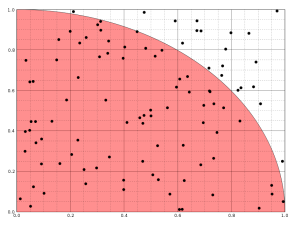
\includegraphics[]{Cercle.PNG}
\end{center}
La première étape de cette exercice consiste a créer une fonction permettant de déterminer si un point est à l'intérieur (zone rouge) ou a l'extérieur du cercle. Puis, générez 10000 points dans cette espace (x et y devrait appartenir à [0,1]). Pour ce faire, vous pouvez utliser la fonction \textit{random.random()} après avoir importé le module \textbf{random}. Vous pouvez obtenir l'approximation de $\pi$ à partir de la formule suivante : $\pi \approx [\frac{\text{Nombre de point dans le cercle}}{\text{Nombre de point total}}]\cdot 4$. Votre réponse devrait être assez proche du vrai chiffre $\pi$.\\
\begin{conseil}
    La fonction random.random() génère aléatoirement un chiffre compris entre 0 et 1. Etant donné que vous devez simulez des points en 2 dimension, vous devrez utiliser 2 fois cette fonction.
\end{conseil}
\begin{solution}
 \lstinputlisting[language = python]{Pi.py}
\end{solution}

\end{Exercice}
\end{document}
